% ============================================================
%  part3/ch14-domain-formation.tex
%  Chapter 14: Domain Formation
% ============================================================

\chapter{Domain Formation}
\label{ch:domain-formation}

\epigraph{%
  Broken symmetry $\rightarrow$ spatial structure.%
}{---}

\begin{WhyChapter}
  Chapter~\ref{ch:phase-transitions} showed that a uniform
  system can have multiple stable ground states.
  This chapter asks what happens when the system is \emph{quenched}:
  rapidly cooled so that different regions select different
  ground states simultaneously.
  The result is spatial domains, interfaces, and coarsening.
  This chapter establishes the coarsening exponents $z = 2$
  and $z = 3$ that will be referenced in every subsequent part.
\end{WhyChapter}


\begin{ChapterIntro}
A system that has just undergone a transition rarely settles immediately into a single coherent state. Instead, different regions make different choices.

One area aligns one way while a neighbouring region aligns another. Boundaries appear. Interfaces form. The system becomes a patchwork of local agreements separated by disagreement.

Many of the structures we observe in nature are not equilibrium states but the frozen remnants of a reconciliation process. The question is not why structure exists, but why some of it persists.
\end{ChapterIntro}

\section{Quenching and domain formation}

After a quench from $T > T_c$ to $T < T_c$, the system
is everywhere in the unstable symmetric state.
Different spatial regions independently begin relaxing toward
$m_+$ or $m_-$.
Where they meet, a domain wall forms.

\begin{definition}[Domain wall]
  A \emph{domain wall} is the interfacial region between two
  regions where $\phi \approx +\phi_0$ and $\phi \approx -\phi_0$.
  Its width scales as $\xi_{\rm wall} \sim \sqrt{\kappa/|r|}$
  where $r = a(T-T_c) < 0$.
\end{definition}

\begin{definition}[Gradient energy functional]
  \label{def:gradient-energy}
  \[
    \mathcal{F}[\Phi]
    = \int\left[W(\Phi) + \frac{\kappa}{2}|\nabla\Phi|^2\right]dx,
    \quad W(\Phi) = \frac{1}{4}(\Phi^2-1)^2.
  \]
\end{definition}

The gradient term penalises interfaces; the double-well
potential $W$ favours $\Phi = \pm 1$.

\section{Allen--Cahn dynamics: non-conserved coarsening}

\begin{definition}[Allen--Cahn equation]
  For a non-conserved order parameter:
  \[
    \partial_t\Phi = -M\frac{\delta\mathcal{F}}{\delta\Phi}
    = M(\kappa\Delta\Phi - W'(\Phi)).
  \]
\end{definition}

\begin{theorem}[Shrinking-circle theorem]
  \label{thm:shrinking-circle}
  \statusproven{}
  Under Allen--Cahn dynamics, a circular domain of radius $R$
  satisfies $R(t)^2 = R_0^2 - 2\kappa M t$, and vanishes at
  time $t^* = R_0^2/(2\kappa M)$.
\end{theorem}

\begin{proof}
  For a circle, $\kappa = 1/R$.
  The interface velocity is $V_n = -M\kappa = -M/R$.
  Since $V_n = dR/dt$:
  $R\,dR = -\kappa M\,dt$.
  Integrating: $\frac{1}{2}R^2 = \frac{1}{2}R_0^2 - \kappa M t$.
  Hence $R(t)^2 = R_0^2 - 2\kappa M t$.
\end{proof}

\begin{theorem}[Allen--Cahn coarsening exponent]
  \label{thm:ac-exponent}
  \statusproven{}
  The characteristic domain size grows as $\ell(t) \sim t^{1/2}$,
  giving dynamic exponent $z = 2$.
\end{theorem}

\begin{proof}
  Interface curvature $\kappa \sim 1/\ell$.
  Interface velocity $V_n \sim \kappa \sim 1/\ell$.
  Since $V_n \sim d\ell/dt$: $d\ell/dt \sim 1/\ell$,
  so $\ell\,d\ell \sim dt$, giving $\ell^2 \sim t$.
\end{proof}

\begin{WorkedExample}[Domain shrinkage]
  A circular domain of radius $R_0 = 10\,\mu{\rm m}$
  with $\kappa M = 1\,\mu{\rm m}^2/{\rm s}$ vanishes at
  $t^* = 100/(2) = 50$ s.
  At $t = 25$ s: $R = \sqrt{100 - 50} \approx 7.1\,\mu{\rm m}$.
\end{WorkedExample}

\section{Cahn--Hilliard dynamics: conserved coarsening}

When the order parameter represents a conserved quantity
(mass, charge, lamphron density), the evolution must preserve
$\int\Phi\,dx$.

\begin{definition}[Cahn--Hilliard equation]
  For a conserved order parameter with chemical potential
  $\mu = \delta\mathcal{F}/\delta\Phi$:
  \[
    \partial_t\Phi = \nabla\cdot(M\nabla\mu)
    = M\Delta(-\kappa\Delta\Phi + W'(\Phi)).
  \]
\end{definition}

\begin{theorem}[Lifshitz--Slyozov coarsening exponent]
  \label{thm:ls-exponent}
  \statusproven{}
  For conserved dynamics, $\ell(t) \sim t^{1/3}$, so $z = 3$.
\end{theorem}

\begin{proof}
  Chemical potential difference between a droplet of radius $R$
  and a flat interface: $\Delta\mu \sim \sigma/R$ (Gibbs--Thomson).
  Diffusive flux to/from the droplet: $J \sim D\Delta\mu/R \sim \sigma D/R^2$.
  Mass conservation: $d(R^3)/dt \sim R^2 \cdot (dR/dt) \sim J \sim 1/R^2$.
  Therefore $dR/dt \sim 1/R^2$, giving $R^3 \sim t$, hence $\ell \sim t^{1/3}$.
\end{proof}

\begin{CrossDomain}[Non-conserved vs.\ conserved coarsening]
  \begin{center}
  \begin{tabular}{@{}lll@{}}
    \toprule
    & \textbf{Allen--Cahn} & \textbf{Cahn--Hilliard} \\
    \midrule
    Conservation & None & $\int\Phi\,dx = $ const \\
    Mechanism & Curvature flow & Ostwald ripening \\
    Exponent & $z = 2$ & $z = 3$ \\
    RSVP field & $\Phi$ (scalar) & $L = \ell^2$ (lamphron) \\
    \bottomrule
  \end{tabular}
  \end{center}
\end{CrossDomain}

\section{Dynamic scaling}

\begin{definition}[Two-point correlation function]
  \[
    C(r,t) = \langle\Phi(x,t)\Phi(x+r,t)\rangle.
  \]
  The characteristic length is defined by
  $C(\ell(t), t) = \frac{1}{2}C(0,t)$.
\end{definition}

\begin{theorem}[Dynamic scaling hypothesis]
  \label{thm:dynamic-scaling}
  For coarsening systems,
  \[
    C(r,t) = f\!\left(\frac{r}{\ell(t)}\right)
  \]
  for a universal scaling function $f$ independent of time.
\end{theorem}

This means the entire time evolution is encoded in the single
growing length $\ell(t)$.

\begin{AdmPreview}
  Dynamic scaling is the coarsening version of admissibility.
  The system ``forgets'' its microscopic initial condition
  and retains only its large-scale domain structure.
  The scaling function $f$ is the admissible reconstruction
  of the system's state from its coarsening length alone.
  This anticipates CLIO (Chapter~\ref{ch:clio}): the optimal
  reconstruction from $\ell(t)$ alone is $f(r/\ell(t))$.
\end{AdmPreview}

\begin{ForwardRef}
  In Part~VII, cosmic voids will be identified with coarsening
  domains and filaments with domain walls.
  The exponent $z_{\rm RSVP}$ will replace $z=2$ or $z=3$
  depending on which dynamical regime dominates.
  Chapters~\ref{ch:scaling-laws} and~\ref{ch:entropy-production}
  develop the phase diagram.
\end{ForwardRef}

\begin{ProblemSet}
\problem{
  Verify Allen--Cahn energy dissipation:
  $\frac{d\mathcal{F}}{dt} = -M\int(\delta\mathcal{F}/\delta\Phi)^2\,dx \leq 0$.
  What is the physical interpretation of the right-hand side?
}
\problem{
  For the Cahn--Hilliard equation, verify mass conservation:
  $\frac{d}{dt}\int\Phi\,dx = 0$ under periodic boundary conditions.
}
\problem{
  A spherical domain of radius $R_0 = 100$ nm coarsens
  under Allen--Cahn dynamics with $\kappa M = 10$ nm$^2$/ns.
  (a) How long until it vanishes?
  (b) If the same domain coarsens under Cahn--Hilliard with
  $D\sigma = 10$ nm$^3$/ns, estimate the time for $R$ to
  halve using the Lifshitz--Slyozov scaling.
}
\problem{
  \textbf{Inverse problem.}
  You observe a two-phase system at time $t = 1000$ s with
  characteristic domain size $\ell = 50$ $\mu$m.
  Can you determine whether the dynamics are Allen--Cahn or
  Cahn--Hilliard from this single observation?
  What sequence of measurements would allow you to determine
  $z$, and what information about the initial state
  is unrecoverable?
}
\end{ProblemSet}

\section{Spinodal decomposition}

\begin{theorem}[Spinodal instability]
  \label{thm:spinodal}
  \statusproven{}
  For conserved dynamics with $f''(\phi_0) < 0$, Fourier modes
  with wavenumber $0 < k^2 < -f''(\phi_0)/\kappa$ grow
  exponentially.
  The homogeneous state is linearly unstable.
\end{theorem}

\begin{proof}
  Linearise $\partial_t\phi = M\Delta(f'(\phi) - \kappa\Delta\phi)$
  around $\phi_0$: set $\phi = \phi_0 + \delta\phi$, giving
  $\partial_t(\delta\phi) = M\Delta(f''(\phi_0)\delta\phi
  - \kappa\Delta\delta\phi)$.
  For Fourier mode $\delta\phi = \hat\phi_k e^{ik\cdot x + \sigma(k)t}$:
  \[
    \sigma(k) = -Mk^2[f''(\phi_0) + \kappa k^2].
  \]
  If $f''(\phi_0) < 0$, then $\sigma(k) > 0$ for
  $k^2 < -f''(\phi_0)/\kappa$.
  These modes grow, generating spontaneous domain formation.
\end{proof}

\begin{WorkedExample}[Spinodal band]
  Let $f''(\phi_0) = -1$ and $\kappa = 0.25$.
  The unstable band is $0 < k^2 < 4$, i.e., $0 < k < 2$.
  The fastest-growing mode is at $k_\star^2 = -f''/(2\kappa) = 2$,
  wavelength $\lambda_\star = 2\pi/\sqrt{2} \approx 4.4$ units.
  Structures spontaneously form at this scale from a uniform state.
\end{WorkedExample}

% ---- Figures ------------------------------------------------

\begin{figure}[ht]
\centering
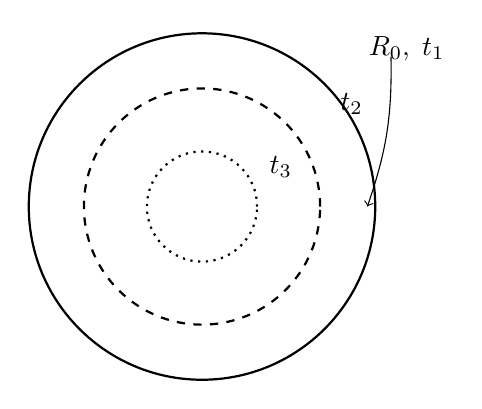
\begin{tikzpicture}
  \draw[thick] (0,0) circle (2.2);
  \draw[thick,dashed] (0,0) circle (1.5);
  \draw[thick,dotted] (0,0) circle (0.7);
  \node at (2.6,2.0) {$R_0,\;t_1$};
  \node at (1.9,1.3) {$t_2$};
  \node at (1.0,0.5) {$t_3$};
  \draw[->] (2.4,1.9) to[bend left=10] (2.1,0);
\end{tikzpicture}
\caption{Allen--Cahn curvature flow: a circular domain shrinks
         according to $R(t)^2 = R_0^2 - 2\kappa M t$
         (Theorem~\ref{thm:shrinking-circle}) and vanishes at
         $t^* = R_0^2/(2\kappa M)$.}
\label{fig:ac-shrink}
\end{figure}

\begin{figure}[ht]
\centering
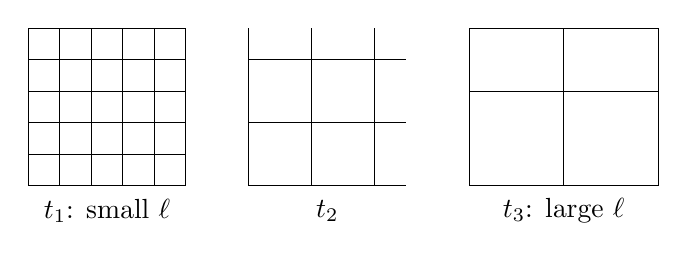
\begin{tikzpicture}[scale=0.8]
  % t1: fine grid representing many small domains
  \foreach \x in {0,0.5,...,2.5} \draw (\x,0)--(\x,2.5);
  \foreach \y in {0,0.5,...,2.5} \draw (0,\y)--(2.5,\y);
  \node at (1.25,-0.4) {$t_1$: small $\ell$};
  % t2
  \foreach \x in {3.5,4.5,5.5} \draw (\x,0)--(\x,2.5);
  \foreach \y in {0,1.0,2.0} \draw (3.5,\y)--(6.0,\y);
  \node at (4.75,-0.4) {$t_2$};
  % t3
  \draw (7,0)--(7,2.5) (7.0,0)--(10.0,0) (10.0,0)--(10.0,2.5)
        (7.0,2.5)--(10.0,2.5) (7,1.5)--(10,1.5) (8.5,0)--(8.5,2.5);
  \node at (8.5,-0.4) {$t_3$: large $\ell$};
\end{tikzpicture}
\caption{Domain coarsening: the characteristic length scale $\ell(t)$
         grows as $t^{1/z}$.
         Domains merge and boundaries disappear over time.}
\label{fig:coarsening}
\end{figure}

\begin{CitationAnchor}
  The Allen--Cahn equation was introduced in Allen \& Cahn~\cite{allen1979}
  to model antiphase boundary motion.
  The Cahn--Hilliard equation for conserved systems was developed
  in Cahn \& Hilliard~\cite{cahn1958}.
  The Lifshitz--Slyozov scaling $\ell \sim t^{1/3}$ originates in
  Lifshitz \& Slyozov (1961).
  The comprehensive review of coarsening dynamics, including both
  $z=2$ and $z=3$ universality classes and dynamic scaling, is
  Bray~\cite{bray1994}, which remains the standard reference.
\end{CitationAnchor}

\begin{FurtherReading}
  Bray (1994) is the essential reference for coarsening dynamics.
  For the mathematical analysis of Allen--Cahn and Cahn--Hilliard
  equations, see Evans~\cite{evans2010} (PDE theory) and
  the review by Elliott (1989).
  Pattern formation more broadly, including spinodal decomposition,
  is treated in Cross \& Hohenberg~\cite{cross1993}.
\end{FurtherReading}
